%Project description
% Problem description
Coupling single-mode fibers to waveguides (Fiber-to-Chip coupling) by microlenses is a very common problem in integrated optics \cite{ integrated_optics}, in wich waveguides locate on a substrate. By means of this technology the simple and reliable optical system with a small size become possible because a lensed fiber has a minized focal length. In this works the application of the lensed fiber-to-chip will be introduced and it coupling efficiency will be discussed.\\
Fig.\quad\ref{fig:experiment_object} is a schematic demonstration of fiber-to-chip coupling. At the one side there is a lensed tapered fiber as laser source and at another side at the working distance of the fiber there is a buried rib waveguide\cite{integrated_optics} as signal receiver. The purpose of this works is to find a way to gain optimized coupling efficiency through the simulations in CST MWS, which is a electromagnetic simulator basically with the implementation of the Finite Integration Technique (FIT)\cite{cst_help_siulation_method}. 


\begin{figure}[!ht]
\centering
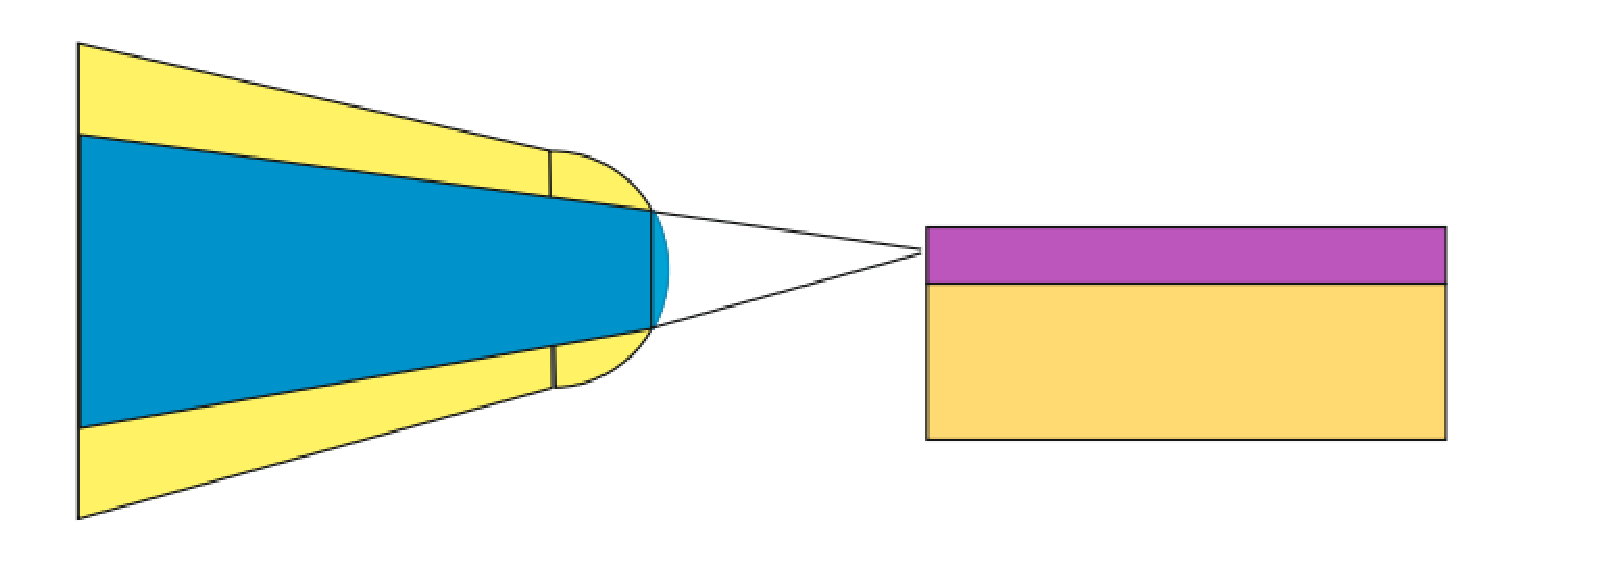
\includegraphics[width=.7\textwidth]{bilder/experiment_object}
\caption{Fiber-to-Chip Coupling}
\label{fig:experiment_object}
\end{figure}

\begin{figure}[!ht]
\centering
\subfigure[Picture of a real Single mode lensed fiber\cite{nanoscal_tapered_fiber}.]{
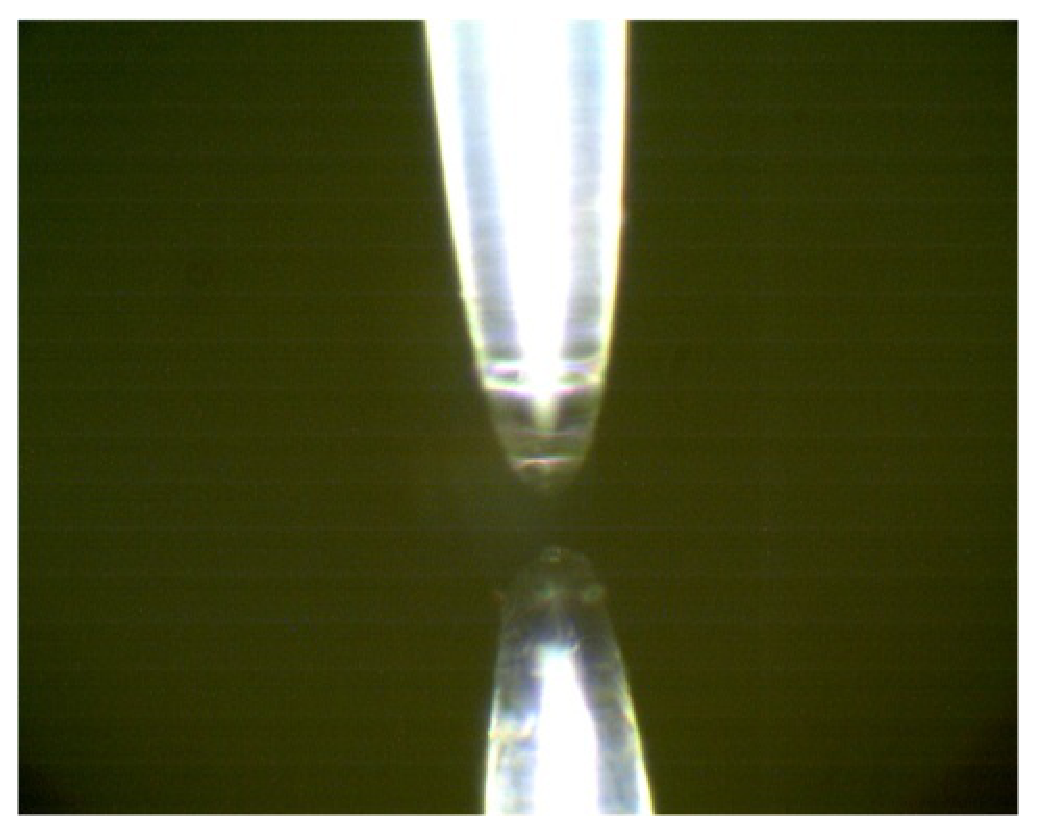
\includegraphics[width=0.3\textwidth]{bilder/single_mode_lensed_fibber}
\label{fig:single_mode_lensed_fiber}
}
\hfill
\subfigure[Schema of a tapered lensed fiber\cite{nanoscal_tapered_fiber}.]{
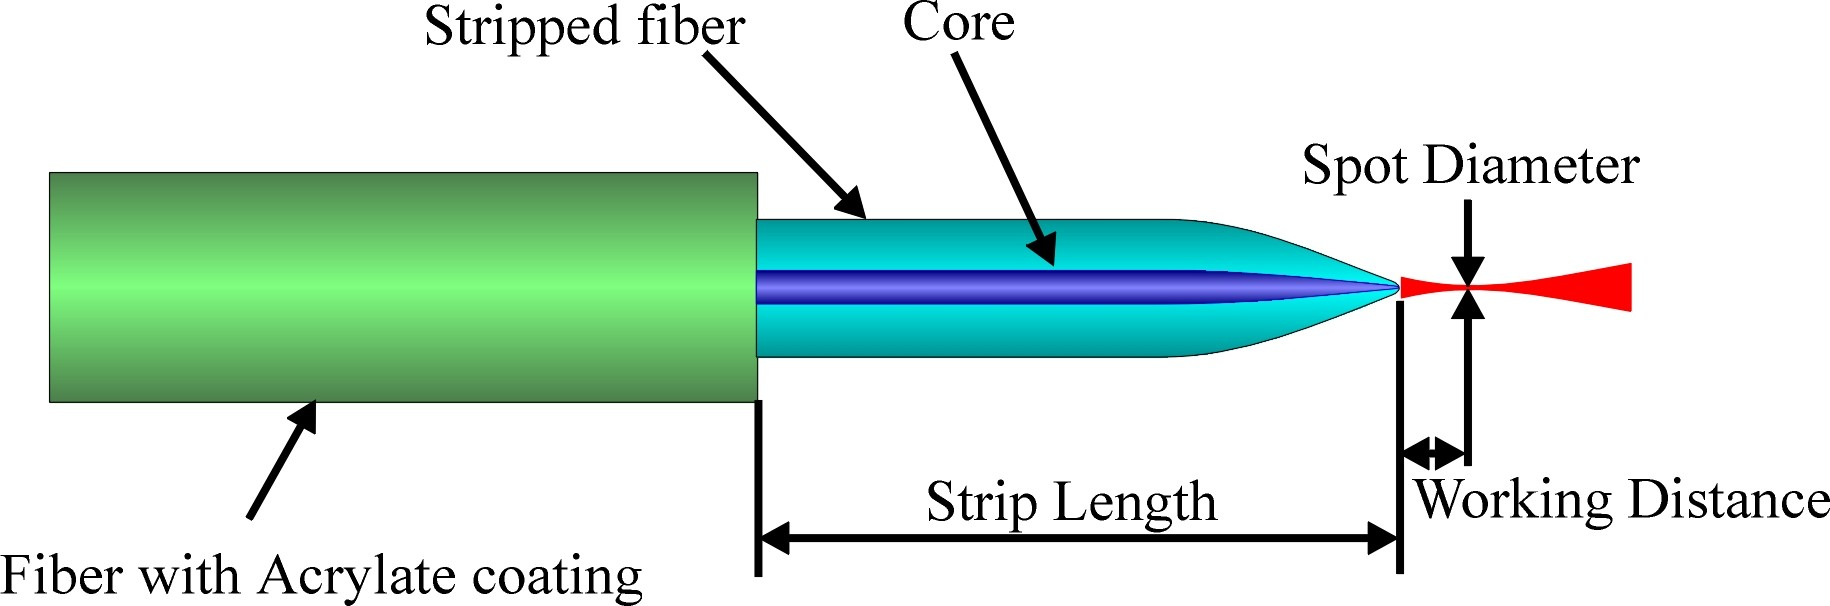
\includegraphics[width=0.6\textwidth]{bilder/tapered_lensed_fiber}
\label{fig:tapered_lensed_fiber}
}
\label{fig:TLFs}
\caption{NANOICS Tapered and Lensed Fibers}
\end{figure}


In this works the the tapered lensed fiber from NANONICS\cite{nanoscal_tapered_fiber} will be used. Fig.\quad\ref{fig:single_mode_lensed_fiber} is the real image of the fiber and Fig.\quad\ref{fig:tapered_lensed_fiber} indicate its schema. In Tab.\quad\ref{tab:technical parameters_lensed_fiber} are listed part of technical parameters, which refer later to the modeling. Additionally the real woking frequence is $\lambda=1064$nm and working distance but $4\mu$m. 
\begin{table}
\caption{Technical parameters about tapered lensed fiber.\cite{nanoscal_tapered_fiber}}
\begin{tabular}{c|c|c}
\hline
\multicolumn{2}{c|}{\textbf{Parameter}}&\textbf{Specification(Single-Mode)}\\
\hline
\multirow{3}{*}{\parbox[t]{0.25\textwidth}{Spot Size of Aspheric and Convex Lenses($1/e^2$)}}&\multirow{2}{*}{Minum}&$1.7\mu$m($\lambda=1.5\mu$m)\\
&																		 &$0.6\mu$m($\lambda=0.6\mu$m)\\
&Maxium															 &$6.0\mu$m($\lambda=1.5\mu$m)\\
\hline
\multirow{2}{*}{Spot Size Tolerance}&\parbox[t]{0.25\textwidth}{Without near-field characterization} &$\pm 0.5\mu$m\\
&\parbox[t]{0.25\textwidth}{With near-field characterization} &$\pm 0.25\mu$m\\
\hline
\multirow{2}{*}{Working Distance} &Minimum &$5\mu$ m($\lambda=1.5\mu$m)\\
&																	Maximum &$50\mu$ m($\lambda=1.5\mu$m)\\
\hline
\end {tabular}

\label{tab:technical parameters_lensed_fiber}
\end{table}

\begin{figure}
\centering
\subfigure[Schema of a real waveguide.]{
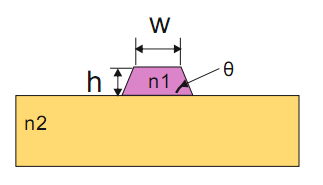
\includegraphics[width=0.4\textwidth]{bilder/orignial_waveguide}
\label{fig:orignial_waveguide}
}
\hfill
\subfigure[Schema of a approxmate waveguide.]{
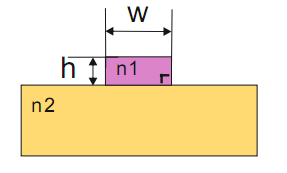
\includegraphics[width=0.4\textwidth]{bilder/approxmate_waveguide}
\label{fig:approxmate_waveguide}
}
\caption{Introduction of  photonic waveguide}
\label{fig:photonic_waveguide}
\end{figure}
The practical waveguide Fig.\quad\ref{fig:orignial_waveguide} is a trapezoid guide on a semiconductor. But the angles $\theta$ of this guide approximate to $90^{o}$ and is not easy to measure because of its micro-size. Thus a simplified guide model Fig.\ref{fig:approxmate_waveguide} will be used in this works. And the detailed technical properties of the photonic waveguide are given:
\begin{itemize}
\item working frequence $\lambda=1064\mu$m
\item guide :LiNbO$_{3}$ with $n1=2.516, w\approx 1\mu$m, $h\approx 0.5 \mu$m
\item substratum: SiO$_{2}$ with $n2=1.544 $
\end{itemize}
